%%%% Document setup
\documentclass[a4paper,landscape,title page]{article}
\setlength{\oddsidemargin}{-0.65in}	% default=0in
\setlength{\textwidth}{11in}		% default=9in
\setlength{\textheight}{6.85in}		% default=5.15in
\setlength{\topmargin}{-1.0in}		% default=0.20in
\setlength{\headsep}{0.35in}		% default=0.35in
\setlength{\parskip}{1.2ex}
\setlength{\parindent}{0mm}

%%%% Use packages
\usepackage{times}
\usepackage{tikz,pgf}
\usetikzlibrary{arrows,automata,trees,plotmarks,calc}


%%%%
\title{Goal-Plan hierarchy for test \textit{testImpactvars3}}
\author{
Dhirendra Singh\\
dhirendra.singh@rmit.edu.au}
\begin{document}
\maketitle

\begin{figure*}[t]
\begin{center}

\begin{tikzpicture}[scale=1.6,level distance=1cm]
\tikzstyle{txt}=[scale=0.9]
\tikzstyle{planbox}=[scale=0.9,draw,minimum height=0.7cm,minimum width=1.2cm]
\tikzstyle{goalbox}=[scale=0.9,draw,rounded corners,minimum height=0.7cm,minimum width=1.2cm]
\tikzstyle{level 1}=[sibling distance=6cm] 
\tikzstyle{level 2}=[sibling distance=8cm] 
\tikzstyle{level 3}=[sibling distance=4.0cm]
\tikzstyle{level 4}=[sibling distance=2.0cm]
\tikzstyle{level 5}=[sibling distance=1cm]

\node[goalbox,yshift=1cm,solid] (T) {$G$}
	child[dashed] {node[planbox] (P1) {$P_1$}}
	child[solid] {node[planbox] (Pi) {$P_i$}
		child {node[goalbox] {$G_{i1}$}
			child {node[planbox] {$P_{i1j}$}
				child {node[goalbox] {$G_{i1j1}$}
					child {node[planbox] {$P_{i1j1k}$} node[txt,below=0.3cm] {$\surd$}}
					child {node[planbox] {$P_{i1j1*}$} node[txt,below=0.3cm] {$\times$}
						edge from parent node[txt,right,near start] {$\times 2$}
					}
				}
				child {node[goalbox] {$G_{i1j2}$}
					child {node[planbox] {$P_{i1j2k}$} node[txt,below=0.3cm] {$\surd$}}
					child {node[planbox] {$P_{i1j2*}$} node[txt,below=0.3cm] {$\times$}
						edge from parent node[txt,right,near start] {$\times 2$}
					}
				}
			}
			child {node[planbox] {$P_{i1*}$}
				child {node[goalbox] {$G_{i1*1}$}
					child {node[planbox] {$P_{i1*1m}$} node[txt,below=0.3cm] {$\times$}}
					child {node[planbox] {$P_{i1*1*}$} node[txt,below=0.3cm] {$\times$}
						edge from parent node[txt,right,near start] {$\times 2$}
					}
				}
				child {node[goalbox] {$G_{i1*2}$}
					child {node[planbox] {$P_{i1*2m}$} node[txt,below=0.3cm] {$\times$}}
					child {node[planbox] {$P_{i1*2*}$} node[txt,below=0.3cm] {$\times$}
						edge from parent node[txt,right,near start] {$\times 2$}
					}
				}
				edge from parent node[txt,right,near start] {$\times 2$}
			}
		}
		child {node[goalbox] {$G_{i2}$}
			child {node[planbox] {$P_{i2j}$}
				child {node[goalbox] {$G_{i2j1}$}
					child {node[planbox] {$P_{i2j1k}$} node[txt,below=0.3cm] {$\surd$}}
					child {node[planbox] {$P_{i2j1*}$} node[txt,below=0.3cm] {$\times$}
						edge from parent node[txt,right,near start] {$\times 2$}
					}
				}
				child {node[goalbox] {$G_{i2j2}$}
					child {node[planbox] {$P_{i2j2k}$} node[txt,below=0.3cm] {$\surd$}}
					child {node[planbox] {$P_{i2j2*}$} node[txt,below=0.3cm] {$\times$}
						edge from parent node[txt,right,near start] {$\times 2$}
					}
				}
			}
			child {node[planbox] {$P_{i2*}$}
				child {node[goalbox] {$G_{i2*1}$}
					child {node[planbox] {$P_{i2*1m}$} node[txt,below=0.3cm] {$\times$}}
					child {node[planbox] {$P_{i2*1*}$} node[txt,below=0.3cm] {$\times$}
						edge from parent node[txt,right,near start] {$\times 2$}
					}
				}
				child {node[goalbox] {$G_{i2*2}$}
					child {node[planbox] {$P_{i2*2m}$} node[txt,below=0.3cm] {$\times$}}
					child {node[planbox] {$P_{i2*2*}$} node[txt,below=0.3cm] {$\times$}
						edge from parent node[txt,right,near start] {$\times 2$}
					}
				}
				edge from parent node[txt,right,near start] {$\times 2$}
			}
		}
	}
	child[dashed] {node[planbox] (P4) {$P_4$}}
;
\node[txt] at ($ (P1)!.5!(Pi) $) {$\ldots$};
\node[txt] at ($ (Pi)!.5!(P4) $) {$\ldots$};

\end{tikzpicture}

\vskip 1.5cm
\caption{Goal-Plan hierarchy for test \textit{testImpactvars3}. There are $2^3$ worlds whose solutions are distributed evenly in each of the $4$ top level plans. Successful execution trace is of length $4$.}
\end{center}
\end{figure*}

\end{document}
%%%%